\documentclass[journal,12pt,two column]{IEEEtran}

\usepackage[utf8]{inputenc}
\usepackage{graphicx}
\usepackage{amsmath}


\title{Assignment 1}
\author{Himanshu Kumar Gupta\\
\textbf{Exercise 3.4, Oppenheimer}}
\date{30 August 2022}


\begin{document}
\maketitle



Consider the z-transform $X(z)$ whose pole-zero plot is as shown in Figure \ref{fig:pole_zero_plt}.
\begin{figure}[!ht]
	\centering
	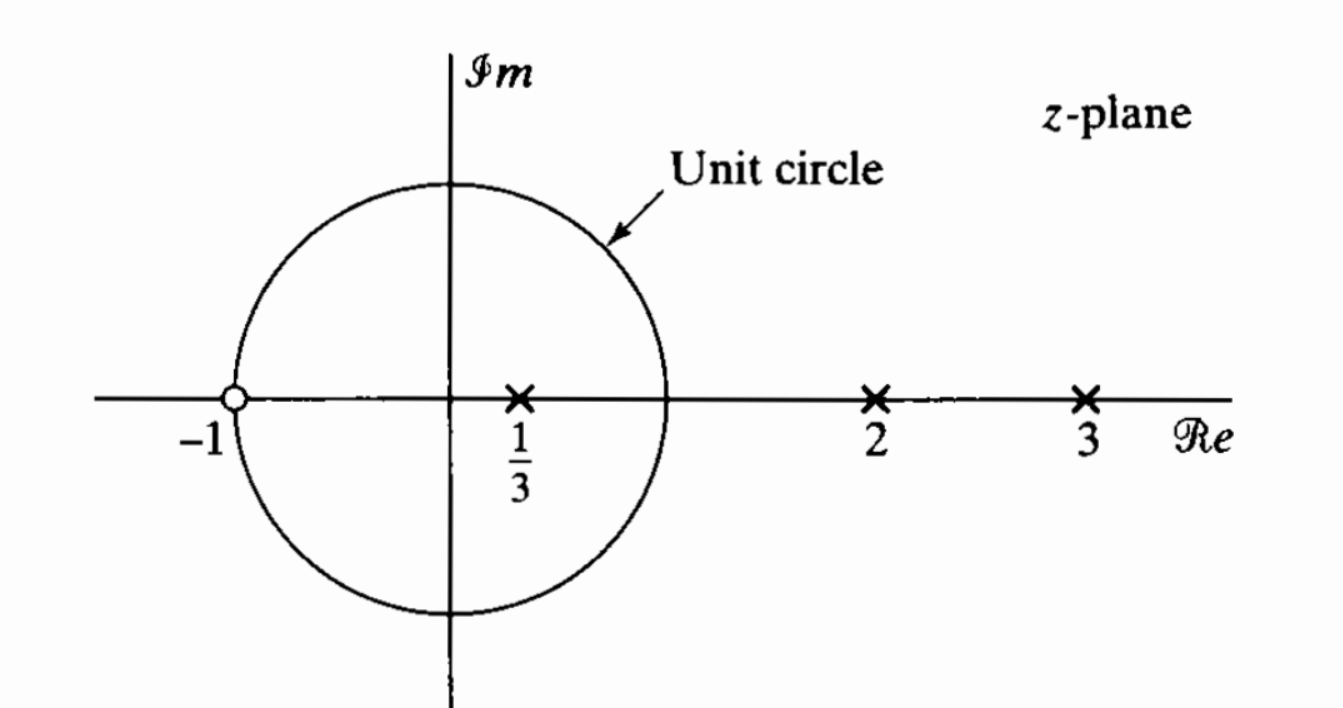
\includegraphics[width=\columnwidth]{./pole_zero_plt}
	\caption{Pole Zero plot of $X(n)$}
	\label{fig:pole_zero_plt}
	\end{figure}
\begin{enumerate}
	\item Determine the region of convergence of $X(z)$  if it is known that fourier transform exists. For this case, determine whether the corresponding sequence $x[n]$ is right sided,left sided, or two sided.
		
		\textbf{Solution} For given figure, 4 ROCs are possible which are
		\begin{align}
		&|x|<|\frac{1}{3}|\\
		|\frac{1}{3}|<&|x|<|2|\\
		|2|<&|x|<|3|\\
		 |3|<&|x|	
		\end{align}
		

		Now,since the fourier transform exist, 
	so the unit circle must lie in ROC. So,
only possible ROC will be $|2|<|x|<|3|$.

		And since its bounded both side by poles only, so the sequence x[n] is two sided.
	\item How many possible two-sided sequences have the pole-zero plot shown in Figure \ref{fig:pole_zero_plt}

		\textbf{Solution} Among 4 ROCs above, we can see that only 2 are bounded both side by poles which are 
		\begin{align}
			|\frac{1}{3}|<|x|<|2|\\  \quad|2|<|x|<|3|
		\end{align}


So,there ar only 2 possible two-sided sequences

	\item Is it possible for the pole-zero plot in Figure \ref{fig:pole_zero_plt} to be associated with a sequence that is both stable and causal? If so, give the appropriate region of convergence.
	
		\textbf{Solution} For stability, ROC must contain the unit circle. So, possible options is 
		\begin{align}
			|\frac{1}{3}|<|x|<|2|
		\end{align}

		For causality, the ROC must be outside of outermost pole which is 3.So, possible option is
		\begin{align}
			|3|<|x|
		\end{align}

		Since nothing is common between two, so there is no possible signal which is both stable and causal.
\end{enumerate}



\end{document}